\documentclass[tikz,border=10pt]{standalone}
\usetikzlibrary{calc}
\begin{document}
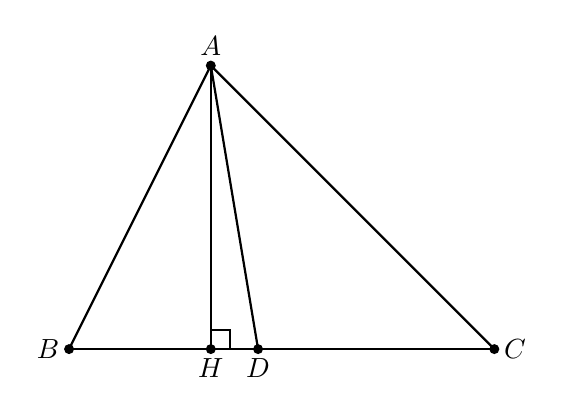
\begin{tikzpicture}[scale=1.2]
  % Coordinates of original figure
  \coordinate (A) at (1.5,3);
  \coordinate (B) at (0,0);
  \coordinate (C) at (4.5,0);
  \coordinate (D) at (2,0);
  % Foot of perpendicular from A to BC
  \coordinate (H) at (1.5,0);

  % Lines of the triangle and segment AD
  \draw[thick] (B) -- (C);
  \draw[thick] (B) -- (A) -- (C);
  \draw[thick] (A) -- (D);

  % New perpendicular segment AH
  \draw[thick] (A) -- (H);

  % Right angle mark at H
  \draw[thick] ($(H)+(0.2,0)$) -- ($(H)+(0.2,0.2)$) -- ($(H)+(0,0.2)$);

  % Dots
  \fill (A) circle (1.5pt);
  \fill (B) circle (1.5pt);
  \fill (C) circle (1.5pt);
  \fill (D) circle (1.5pt);
  \fill (H) circle (1.5pt);

  % Labels
  \node[above] at (A) {$A$};
  \node[left] at (B) {$B$};
  \node[right] at (C) {$C$};
  \node[below] at (D) {$D$};
  \node[below] at (H) {$H$};
\end{tikzpicture}
\end{document}
